\section{AEGIS-Q Design}
\label{sec:design}

\subsection{Planes and trusted state}
\label{sec:design_proc}

Figure~\ref{fig:overall_procedure} separates the persistent secure-storage path from optional accelerator work.  The data plane is an AES-256-GCM block format.  The key-plane workflow contains optional batched ML-KEM envelope refresh for open files; it does not encrypt ordinary file blocks.  The integrity helper computes SHA-256/Merkle material for parity tests and for the committed-prefix anchor root; AEGIS-Q does not persist a per-file content Merkle tree.  The freshness plane publishes an authenticated checkpoint and can target a pre-provisioned TPM NV index; this revision evaluates only fail-closed replay-after-advance behavior for that hardware path.

The design is organized around seven invariants that came directly from the threat model and the review concerns: authenticated key exposure, nonce/generation safety, durable publication ordering, checkpoint exposure, external freshness, unsupported-mode handling, and controller fallback.  Table~\ref{tab:design_goals} is the audit boundary for those invariants.  Each row names the implementation locus, the retained evidence that exercises the invariant, and the narrower paper claim when the current artifact does not close the full production-grade version.

\begin{table*}[t]
\centering
\caption{Formal storage-protocol invariants, implementation loci, retained evidence, and claim boundaries.}
\scriptsize
\setlength{\tabcolsep}{3pt}
\begin{tabularx}{\textwidth}{P{0.20\textwidth}|P{0.27\textwidth}|P{0.25\textwidth}|Y}
\toprule
\textbf{Invariant} & \textbf{Implementation locus} & \textbf{Retained evidence} & \textbf{Claim boundary}\\
\midrule
Envelope authentication before DEK use & \texttt{metadata\_load()} verifies the HMAC-protected envelope before \texttt{pqc\_open()} installs file state & Clean-remount regression and \texttt{user.pqc\_metadata} tamper rejection returning \texttt{EKEYREJECTED} & Remountable authenticated envelope; no hardware-bound credential release\\
AEAD nonce uniqueness & \texttt{derive\_block\_nonce()}, \texttt{build\_block\_aad()}, and \texttt{do\_flush\_wbuf\_locked()} bind file identifier, block, generation, and length & Generation fault matrix, self-test replay regression, clean-remount validation, and daemon cutpoint matrix & Generation-bound record format; physical power loss and broad workload certification remain open\\
Data-before-mapping publication & \texttt{do\_flush\_wbuf\_locked()} writes \texttt{.pqcdata}, calls \texttt{fdatasync}, appends \texttt{.pqcmeta}, then syncs the journal & Journal self-test, daemon cutpoint matrix, and SQLite selected-boundary campaign & D/J ordering evidence; no physical power-loss or drive-cache certification\\
Checkpoint exposure rule & \texttt{logical\_size\_store()}, \texttt{checkpoint\_store()}, \texttt{checkpoint\_load()}, and remount \texttt{ctx\_set()} expose size/checkpoint state only after journal publication & Checkpoint self-test, clean remount, and stale-replay fail-closed artifacts & Authenticated checkpoint exposure; lower-filesystem xattr/directory ordering is delegated\\
External-anchor freshness condition & \texttt{checkpoint\_store()} propagates hardware-anchor failures and \texttt{checkpoint\_load()} rejects mismatched anchor state & TPM NV replay-after-advance run fails closed; file-anchor replay is retained as a negative control & Replay-after-advance freshness only; no persistent PCR-bound lifecycle claim\\
Unsupported-mode boundary & \texttt{pqc\_open()} defaults to FUSE \texttt{direct\_io}; rename and directory \texttt{fsync} return \texttt{ENOTSUP}; internal xattrs are hidden & POSIX scope audit plus current remount/SQLite selected-boundary tests & Ordinary read/write/\texttt{fsync} and narrow disjoint writers only; shared \texttt{mmap} and directory-entry durability are not claimed\\
Controller safety fallback & \texttt{pqc\_block\_job\_choose\_target()} and \texttt{pqc\_admit()} default to CPU on missing slack, stale telemetry, size, deadline, or queue-pressure constraints & Scheduler self-test, admission sweeps, and same-run CUPTI/tegrastats-to-mounted-FUSE throttle traces & Implemented conservative fallback; no foreground inference p99 recovery claim\\
\bottomrule
\end{tabularx}
\label{tab:design_goals}
\end{table*}

\begin{figure*}[t]
  \centering
  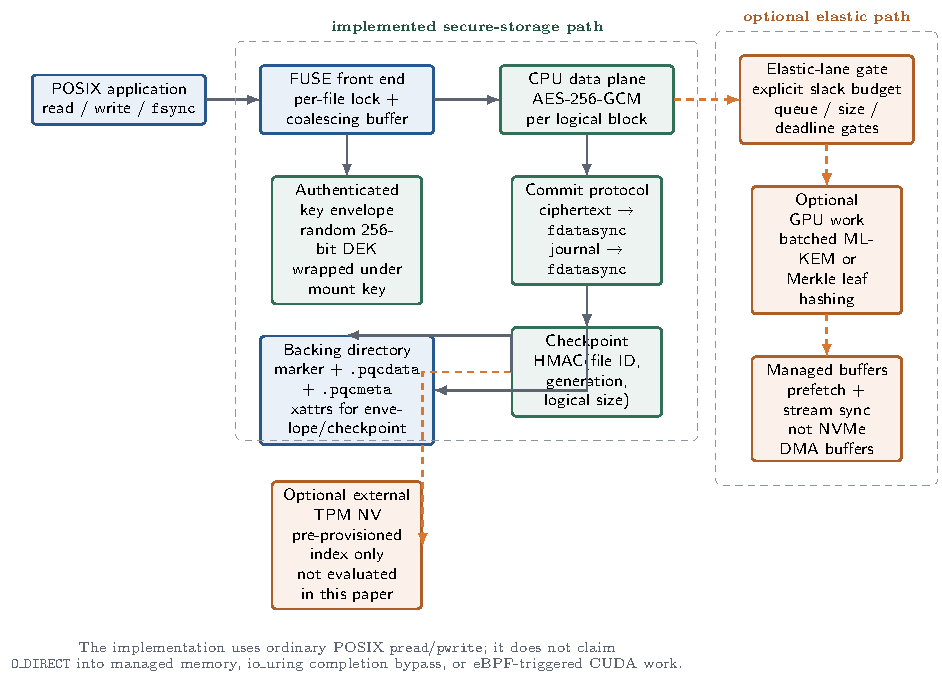
\includegraphics[width=0.98\textwidth]{Figures/fig_architecture.pdf}
  \caption{Implemented AEGIS-Q control and persistence path. Solid arrows are the FUSE format used by the tests; orange dashed arrows denote optional accelerator or externally provisioned hardware paths. The final revision does not claim verified \texttt{O\_DIRECT} UMA pinning, a completed eBPF completion path, or a closed-loop hardware-QoS controller.}
  \Description{Architecture diagram of the AEGIS-Q FUSE data path, key envelope, checkpoint, optional CUDA executor, and optional externally provisioned TPM path.}
  \label{fig:overall_procedure}
\end{figure*}

Mount-key derivation uses PBKDF2 with HMAC-SHA256.  New files receive random 256-bit DEKs and file identifiers; each DEK is masked under mount-key/file-ID material and HMAC-authenticated before open accepts it.  The file identifier, generation, logical block number, and plaintext length are AES-GCM associated data, preventing valid records from moving to different logical positions.

The mount key is password-derived and never hardware-released; there is no hardware-backed credential release path for the mount key.  The rekey is open-file DEK refresh rather than deployed credential rotation: HMAC envelope rewrap for open files; runtime key epoch is in-memory bookkeeping, not a persistent anti-rollback journal.  There is no transactional rewrap recovery claim, and password-derived envelope alone is not rollback resistance; stale old envelopes fail only when generation/checkpoint/external-anchor evidence rejects them.

\subsection{Durable encrypted-block publication}
\label{sec:design_pipeline}

Writes are coalesced only when they are contiguous.  For each affected 4~KiB logical block, AEGIS-Q reads the current authenticated block if necessary, applies the modification, assigns a strictly increasing generation, and derives the GCM nonce from \((\mathit{fileID},\mathit{block},\mathit{generation})\).  The commit order is:

\begin{enumerate}
  \item write ciphertext records to \texttt{.pqcdata} and call \texttt{fdatasync};
  \item append generation-to-offset mappings and tags to \texttt{.pqcmeta}, then call \texttt{fdatasync};
  \item update the logical-size xattr; authenticate and write the checkpoint.
\end{enumerate}

Figure~\ref{fig:djc_state_machine} makes the publication state machine explicit.  It is intentionally not a proof diagram: the transition table records which edges are exercised by retained artifacts and which crash boundaries remain outside the evaluated envelope.

\begin{figure*}[t]
\centering
\scriptsize
\begin{tikzpicture}[
  node distance=0.45cm and 0.55cm,
  state/.style={draw, rounded corners, align=center, minimum width=1.65cm, minimum height=0.48cm, inner sep=2pt},
  edge/.style={->, thick}
]
\node[state] (clean) {clean\\mount};
\node[state, right=of clean] (data) {data record\\durable};
\node[state, right=of data] (journal) {journal mapping\\durable};
\node[state, right=of journal] (ckpt) {checkpoint/\\xattr exposed};
\node[state, right=of ckpt] (anchor) {anchor update\\attempted};
\node[state, right=of anchor] (remount) {remount\\validated};
\node[state, below=0.55cm of journal] (stale) {stale generation\\observed};
\node[state, right=of stale] (closed) {latest state or\\fail-closed read};
\draw[edge] (clean) -- node[above] {\texttt{write}} (data);
\draw[edge] (data) -- node[above] {\texttt{fdatasync}} (journal);
\draw[edge] (journal) -- node[above] {gen+ckpt} (ckpt);
\draw[edge] (ckpt) -- node[above] {anchor} (anchor);
\draw[edge] (anchor) -- node[above] {open/read} (remount);
\draw[edge] (journal) -- node[left] {replay} (stale);
\draw[edge] (stale) -- node[above] {oracle} (closed);
\end{tikzpicture}
\vspace{2pt}
\begin{tabularx}{0.98\textwidth}{P{0.18\textwidth}|P{0.21\textwidth}|P{0.30\textwidth}|Y}
\toprule
\textbf{Transition} & \textbf{Boundary label} & \textbf{Retained artifact} & \textbf{Scope}\\
\midrule
clean mount $\rightarrow$ data durable & write syscall boundary + generation assignment & generation matrix partial-update row and daemon data-write SIGKILL row & One-block daemon evidence; multi-block application atomicity requires an app journal\\
data durable $\rightarrow$ journal durable & \texttt{fdatasync(.pqcdata)}; crash cut point before J & daemon journal-append/fsync rows and SQLite selected-boundary campaign & Selected cutpoints only; not a physical power-loss proof for all filesystems\\
journal durable $\rightarrow$ checkpoint/xattr exposed & journal \texttt{fdatasync}/\texttt{fsync}; generation update and checkpoint field authenticated & checkpoint self-test and clean-remount artifacts & Lower-filesystem xattr atomicity and directory durability are delegated\\
checkpoint/xattr $\rightarrow$ anchor attempted & checkpoint field authenticated; anchor update attempted & TPM replay-after-advance fail-closed artifact; file-anchor negative control & Hardware freshness only after provisioned NV anchor; no persistent PCR lifecycle\\
remount validation $\rightarrow$ read decision & envelope/checkpoint authenticated, mapping selected, AEAD tag checked & tamper rejection, clean remount, generation matrix rows & Validated read/write/\texttt{fsync} envelope; unsupported POSIX modes remain open\\
stale generation $\rightarrow$ latest or fail closed & highest-generation lookup plus AEAD generation binding; oracle verdict & older-generation append row and self-test regression & Replayed mapping does not supersede newer mapping; broad crash certification remains open\\
\bottomrule
\end{tabularx}
\caption{D/J/C/xattr publication state machine and transition audit.  D is the durable ciphertext sidecar state, J is the journal mapping state, and C is the authenticated checkpoint/logical-size exposure state.}
\Description{A state-machine diagram from clean mount through data durability, journal durability, checkpoint exposure, anchor update, remount validation, and stale-generation rejection, with a transition table linking each edge to retained artifacts and scope.}
\label{fig:djc_state_machine}
\end{figure*}

The journal is the publication point: a ciphertext tail with no durable mapping is unreachable after recovery.  Conversely, a mapping is written only after its ciphertext range has crossed the data durability barrier.  \texttt{fsync} flushes the coalescing buffer, waits for local pending work, and calls \texttt{fdatasync} on both sidecars before returning.  This is an implementation argument for the tested format, not a proof of full POSIX behavior under every FUSE cache mode or an SQLite certification.

The generation rule is intentionally simple.  A generation value is consumed when a new record is constructed for a logical block; recovery accepts only records reachable through a validated mapping and checkpoint.  Reusing an older generation for a new plaintext would be a correctness bug because the GCM nonce is derived from file identifier, block, and generation.  The retained generation matrix exercises partial update, clean remount, torn journal tail, stale snapshot replay, and an adversarial older-generation append after a newer mapping; the daemon cutpoint matrix adds selected one-block SIGKILL timing.  The paper still does not claim physical power-loss or broad crash-consistency certification.

Unsupported POSIX modes are part of the design boundary.  The retained audit confirms the implemented contract: ordinary read/write/\texttt{fsync} and narrow disjoint writers are supported; default encrypted-file \texttt{mmap}, rename, and directory \texttt{fsync} are rejected; internal checkpoint/envelope xattrs are hidden; and FUSE writeback-cache/direct-IO mmap capabilities are not requested.  Arbitrary conflicting concurrency and directory-entry durability remain outside the claim.

\subsection{Managed-memory boundary and scheduler}
\label{sec:design_uma}

Table~\ref{tab:memory_compat} summarizes the claims that the source code actually makes: accelerator placement must be subordinate to storage correctness, CPU/GPU ownership is protected by the FUSE per-file lock and stream completion, and CUDA prefetch is used only to influence locality.  No table entry is a statement about NVMe page pinning, cache coherence of a third-party DMA engine, or CUDA attach-mode permissions.

\begin{table}[t]
\centering
\caption{Memory-path claims and their hardware-verified status.}
\scriptsize
\setlength{\tabcolsep}{3pt}
\begin{tabularx}{\columnwidth}{P{0.38\columnwidth}|P{0.20\columnwidth}|Y}
\toprule
\textbf{Mechanism} & \textbf{Status} & \textbf{Claim retained}\\
\midrule
\texttt{cudaMallocManaged} + prefetch & Verified & Managed allocation and explicit device/host prefetch complete.\\
\texttt{posix\_memalign} + \texttt{cudaHostRegister} & Prototype-only & Host-memory pinning and executor-local access checks; not a verified storage-DMA path.\\
\texttt{pread}/\texttt{pwrite} sidecars & Verified & Backing ciphertext and journal use ordinary POSIX I/O.\\
eBPF tracepoint notification & Not claimed & No final eBPF notification path is part of the verified implementation.\\
QoS telemetry & SQLite recovery only & Workload/CUPTI traces can drive mounted-FUSE throttling; no foreground AI p99 recovery claim.\\
\bottomrule
\end{tabularx}
\label{tab:memory_compat}
\end{table}

The placement function balances workloads between the ARM CPUs and the Jetson GPU. The current revision does not expose a verified \texttt{O\_DIRECT} storage path into GPU memory.  The CUDA executor instead uses managed allocation, explicit prefetch, and stream synchronization as locality and ordering controls.

QoS follows the SQLite contract in Figure~\ref{fig:first_page_qos}: secure-storage pressure raises AEGIS-Q p99 from 6.4~ms to 13.8~ms; classification recovers 8.8~ms, zero deadline misses, and 2.7~MB/s background progress, not foreground-inference p99 or completion-bypass control.

The producer-facing interface is deliberately conservative.  A job can enter the elastic lane only when its size and batch shape make GPU execution plausible and the producer supplies nonzero relative slack in nanoseconds.  The trace records \texttt{CLOCK\_REALTIME} timestamps for correlation; batch age, deadline, and slack age are \texttt{CLOCK\_MONOTONIC}-relative and need no cross-process clock synchronization.  Missing, zero, or stale slack falls back to CPU with the exact deferral reason.  The mounted path also exposes \texttt{user.pqc\_qos\_class}: latency files are traced but never daemon-slept, elastic files are throttle-eligible, and SQLite sidecars inherit the base-file class.

The evaluated key-plane workflow applies this rule by batching open-file descriptors, encapsulating on the selected executor, installing 32-byte refreshed DEK material, and rewriting the HMAC-authenticated envelope.  It is not a persistent KEM hierarchy or hardware-backed credential lifecycle.

\subsection{Freshness boundary}
\label{sec:design_security}

The file anchor is an authenticated on-disk record.  Because an attacker able to restore the backing directory can restore that record as well, it is explicitly \emph{not} rollback protection.  The crash/replay harness treats this behavior as a negative control.  The optional hardware backend refuses to mount when its TPM NV index was not provisioned by an administrator; it never creates persistent TPM state implicitly.  The retained hardware evidence is narrower: replay after the anchor advances fails closed.  A stronger rollback-resistance claim requires a separately protected TPM policy, defined NV authorization, a recovery protocol, and power-loss results for that exact configuration.
